\documentclass[]{interact}
\usepackage{epstopdf}% To incorporate .eps illustrations using PDFLaTeX, etc.
\usepackage{subfigure}% Support for small, `sub' figures and tables
%\usepackage[nolists,tablesfirst]{endfloat}% To `separate' figures and tables from text if required

\usepackage{natbib}
\bibliographystyle{chicago}
\setcitestyle{authoryear,open={(},close={)}}
\renewcommand\bibfont{\fontsize{10}{12}\selectfont}% Bibliography support using natbib.sty

\usepackage{hyperref}
\hypersetup{
    colorlinks=true,
    linkcolor=blue,
    filecolor=magenta,
    urlcolor=blue,
    citecolor=blue,
}

\usepackage{titlesec}
\titleformat*{\section}{\Large\bfseries}
\titleformat*{\subsection}{\large\bfseries}

\usepackage{endnotes}
\let\footnote=\endnote
\usepackage{etoolbox}
\patchcmd{\enoteformat}{1.8em}{0pt}{}{}

\theoremstyle{plain}% Theorem-like structures provided by amsthm.sty
\newtheorem{theorem}{Theorem}[section]
\newtheorem{lemma}[theorem]{Lemma}
\newtheorem{corollary}[theorem]{Corollary}
\newtheorem{proposition}[theorem]{Proposition}

\theoremstyle{definition}
\newtheorem{definition}[theorem]{Definition}
\newtheorem{example}[theorem]{Example}

\theoremstyle{remark}
\newtheorem{remark}{Remark}
\newtheorem{notation}{Notation}

\usepackage{tabularx}
\usepackage{booktabs,caption}
\usepackage{threeparttable}

\usepackage{lscape}
%%%%%%%%%%%%%%%%%%%%%%%%%%%%%%%%%%%%%%%%%%%%%%%%%%

\begin{document}

\articletype{DRAFT MANUSCRIPT}

\title{Replication Survey}

\author{
\name{Peter Kedron\textsuperscript{a,b}\thanks{CONTACT Peter Kedron. Email: Peter.Kedron@asu.edu}, Joseph Holler\textsuperscript{c}, and Sarah Bardin\textsuperscript{a,b}}
\affil{\textsuperscript{a}School of Geographical Sciences and Urban Planning, Arizona State University, Tempe, Arizona, USA; \textsuperscript{b}Spatial Analysis Research Center (SPARC), Arizona State University, Tempe, Arizona, USA; \textsuperscript{c}Department of Geography, Middlebury College, Middlebury, Vermont, USA}
}

\maketitle

\begin{abstract}
Write Abstract

\end{abstract}

\begin{keywords}
Reproducible Research, Epistemology, Geographic Research Methods
\end{keywords}

%%%%%%%%%%%%%%%%%%%%%%%%%%%%%%%%%%%%%%%%%%%%%%%%%%
\newpage
\section*{Introduction}
Since the 1600s, replication has been a defining characteristic of the scientific method and an essential tool of researchers working to remove errors from our understanding of phenomena. 
\citet{nosek2020} broadly define a replication as any study that has at least one outcome that would be considered to be diagnostic evidence of a claim from prior research.
More frequently, replication is defined along two axes that help to distinguish the type of diagnostic evidence a study will provide and the function or purpose it is intended to serve. 
First, it is common to distinguish whether a replication study used the same data as the original study, or if new data were collected and analyzed. 
Second, it is helpful to identify whether a replication is focused on the question of whether the specific results of the original study can be reobserved, or whether the conclusions drawn from the original study are robust to changes in procedure or context.

When a researcher asks whether the same data and procedures can be used to generate the same results as an original study the central purpose of their study is verification.
If the researcher uses the original data, but introduces procedural differences they think may effect the original result they pursue a reanalysis designed to determine whether the original reasoning was somehow erroneous. 
Both of these approaches to replication assess the internal validity of research and are more commonly referred to as reproductions.
If the researcher tries to follow the procedures of an original study, but collects new data, the purpose shifts to evaluating the external validity of the original result by retesting it under new conditions.
This approach is commonly referred to as replication. 

While a replication or reproduction can never provide conclusive evidence for or against a finding, either type of study can be informative. 
If a well-executed, high-quality replication or reproduction recreates the result of an original study, we are apt to increase our confidence in the original findings. 
If a finding cannot be recreated, it reduces our confidence in the original result and suggests that our current understanding of the system being studied or our methods of testing that system are insufficient.

For example, in a survey of 807 ecologists and evolutionary biologists, 64 percent admitted to failing to report non-significant results and 51 percent admitted to presenting unexpected findings as if they had been hypothesized from the start of the research \citep{fraser2018questionable}.

%%%%%%%%%%%%%%%%%%%%%%%%%%%%%%%%%%%%%%%%%%%%%%%%%%
\section*{Data and Methods}
Complete documentation of the procedures, survey instrument, and other materials used in this study are available through the Survey of Researcher Perceptions of Replication in Geography Repository (OSF WEBSITE).
The repository connects to a GitHub repository which hosts the anonymized dataset and code used to create all results and supplemental materials along with a complete history of their development. 
All of the results presented in this paper can be independently reproduced using the materials in that repository.
Before the start of data collection, we registered a preanalysis plan for the survey with OSF Registries (\citet{Kedron_RPl_Survey_PAP} - \url{https://osf.io/a4nwg}). 
The survey was conducted under the approval and supervision of the Arizona State Institutional Review Board - \textit{STUDY00014232}.

%%%%%%%%%%%%%%%%%%%%%%%%
\subsection*{Sampling Frame}
Our target population of interest is researchers who have recently published in the field of geography. 
We followed a 4-step procedure to create a sampling frame for our survey that captures this diverse population of researchers. 

First, beginning at the publication level, we identified journals indexed as either geography or physical geography by the \href{https://access.clarivate.com/}{Web of Science's Journal Citation Reports} that also had a 5-year impact factor greater than 1.5.
From those journals, we created a database of all articles published between 2017 and 2021.  

Second, we used Arizona State University's institutional subscription to the \href{https://www.scopus.com/home.uri}{Scopus Database} to extract journal information (e.g., subject area, ranking), article information (e.g., abstract, citation counts), and author information (e.g., corresponding status, email) for each publication. 
Because our intention was to capture individuals actively publishing new geographic research, we retained publications indexed by Scopus as \textit{document type = ``Article''} and removed all other publication types (e.g., editorials, book reviews) from our article database. 
We also removed articles with missing authorship information. 

Third, we created a list of researchers and their published articles, focusing on corresponding authors for two reasons.
(1) Corresponding authorship is one indicator of the level of involvement an individual had in a given work. 
While imperfect, it was the best available indicator in the Scopus database as across journals there is no commonly adopted policy for declarations of author work (e.g., CRediT Statements).
(2) Scopus maintains email contact information for all corresponding authors, which gave us a means of contacting researchers in our sampling frame.
Scopus also maintains a unique identifier for each author (author-id) across time, which allowed us to identify authors across publications. 

Fourth, we constructed a sampling frame of unique researchers and their most recent email contact information. 
We determined uniqueness by grouping researchers by their author-id, and we determined the most recent contact information by selecting records associated with the most recent year of publication. 
For 383 researchers who had two or more distinct emails in the latest year of publication, we removed non-institutional personal email addresses and then selected one of the remaining institutional email address.

Applying these criteria yielded a sampling frame of 29,828 researchers. 
On average, these authors published 2.7 articles in geography journals meeting our criteria between 2017 and 2021. 
Roughly one-third (33.0\%) were most recently a corresponding author for an article published in a general geography journal. 
A similar proportion (32.0\%) were most recently a corresponding author for an article published in an earth sciences journal, and smaller proportions had published in the social sciences and cultural geography (20.0\% and 16.0\%, respectively).

\subsection*{Survey Instrument}
The survey first established eligibility based on age and geographic research activity in the past five years and asked researchers to report their primary subfield and methodology.
We asked each participant to assess their familiarity with the term ``replicability'' and to provide their own definition. 
We then provided a definition based on the \citet{nosek2020replication}  to establish a common understanding of replicability for the remainder of the survey.
Remaining questions assessed the epistomological purpose of a replication (5 questions), factors that impact the chances of successfully replicating a study (18 questions) or the decision to attempt a replication (13 questions), and what portion of the geographic literature has/could/should be replicated (3 questions).
For researchers who reported attempting reproductions, we asked researcher to elaborate on their motivations and outcomes (9 questions).

We developed the survey questions following a review of prior reproducibility surveys \citep[e.g.,][]{fanelli2009many,baker20161, konkol2019} and our own reading of recurring issues in the reproducibility and replicability literature. 
We pilot tested the survey instrument with \textit{n}=19 graduate students and geography faculty with differing levels of experience, topical focus, and methodological background. 
After pilot testing, we removed these individuals from our sampling frame to ensure they would not be included in our final sample.

%%%%%%%%%%%%%%%%%%%%%%%%
\subsection*{Data Collection}
We used a digital form of the Tailored Design Method \citep{dillman2014internet} to survey geographic researchers between May 17 and June 10, 2022.
A simple random sample of 2,000 researchers was drawn without replacement from our sampling frame, and those researchers were invited via email to participate in the online survey. 
Researchers received their initial invitation on May 17, 2022. 
Two reminder emails were sent to researchers that had not yet completed the survey on May 26 and May 31, 2022.

The online survey was administered through \href{https://www.qualtrics.com/}{Qualtrics}. 
Participation in the survey was entirely voluntary. 
Each researcher that opted to participate in the survey was provided with IRB approved consent documentation and linked to the internet survey instrument. 
Participants were also given the option to provide an email address for eligibility for one of three  prizes of 90 US\$, selected randomly after the data collection period.
Participating researchers had the option to exit and re-enter the survey and were also able to review and change their answers using a back button as they progressed through the survey.
At the end of the data collection period, responses were checked for completeness and coded using the reporting standards of the American Association For Public Opinion Research \citep{aaporstandards}.
Responses were downloaded from Qualtrics, anonymized, and stored in a public de-identified database in the research compendium (self-identifying reference removed).


%%%%%%%%%%%%%%%%%%%%%%%%%%%%%%%%%%%%%%%%%%%%%%%%%%
\section*{Results}
A total of \textit{n}=283 of the authors we contacted completed the online survey with information sufficient for analysis. 
The contact rate for the survey was 18.8 percent, the response rate was 14.1 percent, yielding a cooperation rate of 74.4 percent. 
The refusal rate was 4.8 percent\endnote{All outcome rates are reported using \citet{aaporstandards} standards. 
The outcome rates used were - response rate 2, cooperation rate 2, refusal rate 1, and contact rate 1.}.
Respondents were predominantly male (65.1\%) and between the ages of 35 and 55 (62.4\%). 
The majority of respondents were also academics, but were well balanced across career levels as no one category made up more that 30 percent of the sample.
Respondents were similarly balanced across disciplinary subfields, but did contain a greater number of physical geographers  - human geography (26.8\%), physical geography (39.9\%), nature and society (14.8\%), geographic methods and GIScience (17.3\%). 
Different methodological approaches were well represented by respondents in the sample with qualitative researchers making up the smallest sub-group  - quantitative (47.3\%), qualitative (16.3\%), and mixed-methods (36.0\%).

%%%%%%%%%%%%%%%%%%%%%%%%
\subsection*{Researcher Definitions of Replication and its Epistemic Functions}
\begin{itemize}
    \item Respondents report thinking about replicability (73.9\%) talking with colleagues about replicability (65.0\%) and considering replicability when undertaking peer-review (59.0\%). 
    \item Far fewer respondents report attempting replications (31.8\%). 
\end{itemize}

\begin{itemize}
    \item Coded analysis of Q6
\end{itemize}

A majority of respondents believe replications can serve epistemic functions.
\begin{itemize}
    \item Q7 control of chance 64.5\%
    \item Q7 identify product of flawed design 59.7\%
    \item Q7 construct validity 75.2\%
    \item External validity population 62.9\%
    \item External validity location 67.8\%
    \item Human, Nature Society, and Qualitative researchers had lower agreement on each point.
\end{itemize}

%%%%%%%%%%%%%%%%%%%%%%%%
\subsection*{Replication - Chances and motivations}
Overall respondents believe that the majority of research in the discipline has not been independently replicated and appear to be uncertain about what proportion of the literature could or should be replicated (Figure \ref{fig:Q12-HCS}). 
On average, respondents estimated that 25 percent of recent studies in their sub-field have be replicated. 
However, the distribution of these responses is strongly right skewed.
In fact, 46.9 percent of respondents estimated that less than 10 percent of recent studies have been replicated.
It is unclear if respondents believe recent geographic research could or should be replicated.
On average, respondents estimated that approximately half of studies 'could be replicated' (55.0\%) or 'should be replicated' (55.9\%). However, the distribution of responses to both questions are relatively flat across the range of possible values and highly variable (\textit{$sd_{could}=24.3\%$}, \textit{$sd_{should}=27.7\%$}), which suggests 
respondents were uncertain whether it was possible or valuable to replicate recent research.  

\begin{center}
\textbf{Insert Figure \ref{fig:Q12-HCS} About Here}
\end{center}

Respondents identified a range of factors that might impact the chances of an independent researcher replicating the claims of a prior study (Figure \ref{fig:Q8-10-Chances}a).
A majority of respondents identified the transparency and availability of the components of a study as affecting the odds of replication. 
Poor documentation of the original study (75\%) and the use of restricted access data (68\%) were seen by the greatest number of respondents as decreasing the odds of replication. 
Some respondents identified the inclusion of multiple sites in a study as increasing the chances of an independent replication of the findings of that study, but not in great enough numbers to constitute a majority. 

The characteristics of the research team that conducted the original study were generally not identified by respondents as likely to change the changes of replicating that study. 
Respondents were nearly evenly split as to whether a large research team working on a study increased of decreased the chances of replicating that study. 
On the whole, more respondents believed that reliance on the unique expertise of the research team conducting a study, or the position adopted by that team would decrease, rather than increase, the chances of replicating the claims of a study.
However, only 54 percent of respondents thought the position a research team chose to adopt when conducting study would decrease the chances of replicating that study. 
Similarly, 49 percent of respondents identified reliance on the unique expertise of the original researcher team as decreasing the odds of replicating a study. 


\vspace{5mm}


Researcher identified more study characteristics than phenomena characteristics, which may indicate they they are thinking of this through the lens of artifact availability from the prior study and not the nature of the phenomena. 
A small but notable percentage of researchers indicated that they simply did not know whether a factor would affect chances of replication. 


Only a subset of study characteristics were consistently identified by geographic researchers as altering the chances of replicating the claims of a prior study.
\begin{itemize}
    \item Agreement that quantitative studies are more likely to be replicable (80.6\%)
    \item Minimal variation in responses across method groups or sub-fields. 
\end{itemize}

Phenomena
\begin{itemize}
    \item Spatial dependence lean to decrease chance of replication (41.0\%), but notable percentage of respondents (21.6\%) indicated not having a clear idea of whether this would matter.
    \item Belief that strong relationship between a phenomenon and local conditions reduced chances of replication (59.7\%)
    \item Fairly even spread across increase, decrease, no effect on exhibits variation across space.
    \item When a phenomenon cannot be directly measured decreases chance of replication (61.5\%).
    \item Really even distribution on nearly a phenomenon characteristics. Also a decently high percentage of i don't know resposnes for each characteristic. In most cases in the 10-20 percent range. 
\end{itemize}


\begin{center}
\textbf{Insert Figure \ref{fig:Q8-10-Chances} About Here}
\end{center}

%%%%%%%%%%%%%%%%%%%%%%%%
\subsection*{Factors that Affect the Decision to Attempt Replications}
Several factors appear to affect whether researchers decide to attempt to replicate recent geographic research.
Figure \ref{fig:Q15-DecisionFactors} presents how frequently respondents believe differences in academic incentives (AI), the availability of research artifacts (AA), and study characteristics (SC) affect researchers' decisions to attempt to replicate existing geographic research.
Response characteristics for each factor are recorded at the right of the figure.

\begin{center}
\textbf{Insert Figure \ref{fig:Q15-DecisionFactors} About Here}
\end{center}

Geographic researchers identified current academic incentives as the factor most frequently impacting the decision to attempt a replication study. 
A majority of respondents identified the pressure to publish original research (77\%) and the lack of funding for replication studies (73\%) as frequently or always impacting the decision to attempt a replication.
Respondents also believed that the perception of replications as low value work (64\%) that was often difficult to publish (63\%) also impacted decision making.  
Contrary to some narratives in the replication literature, the desire to identify fabricated data or results was not seen as a determining factor in the decision to attempt a replication. 
However, this finding should be interpreted with caution as a third of respondents indicated that they did not know whether potential fabrication influenced researcher decision making.  

Respondents also identified the availability of research artifacts as important to the decision to attempt a replication study.
Respondents believe that difficulty accessing and recreating data (61\%) frequently or always affects the replication decision.
Similarly, a slight majority of respondents (51\%) identified the accessibility of procedural and methodological information as a influential factor. 
The challenge of recreating the methods of a prior study elicited a similar response (47\%).

No characteristics of the original study, or the potential replication attempt, were identified by a majority of researchers as frequently or always impacting the replication decision. 
However, a near majority of respondents did identify potential geographic variation in the phenomena being investigated (43\%) and inexperience conducting replication studies (45\%) as influencing decisions to attempt replications. 
Respondents did not see a low chance of successfully replicating a study as a deterrent to attempting a replication, but it is unclear whether this result is driven by a belief in the value of null replication results, or the belief that replications in fact have high chances of success.
Finally, respondents did not identify ethical concerns as a factor affecting the decision to attempt a replication study. 

Respondents identified a number of factors that were omitted from our survey instrument as important when deciding whether to attempt a replication of a geographic study. 
These factors include practical issues such as the difficulty identifying and accessing new field sites where data would be collected during a replication attempt, the costs of conducting a replication, and the time needed to obtain institutional approvals.
Respondents also identified uncertainty about how to compare the results of a replication attempt to the original as important to the replication decision.. 
Finally, a small number of respondents believe that geographic researchers do not undertake replication studies because those researchers either believe replication is not possible or not necessary in geography. 
These respondents argued that the main value of geographic studies is that each study provide a unique lens on the portion of the world under investigation, which makes replication a unnecessary endeavour.   

Respondents from different disciplinary sub-fields and methodological approaches varied little in their identification of the factors affecting researchers' decisions to attempt replication studies. 
Human geographers and researchers using quantitative methods less frequently identified academic incentives as important to the replication decision when compared to other sub-groups, but were otherwise broadly similar in their views on artifact availability and study characteristics. 
A greater percentage of quantitative researchers and those working in the areas of GIScience and Methods identified the accessibility of data and methodological information as more often impacting the decision to replicate, but not at a level that was substantially higher than other sub-groups. 
In fact, a greater percentage of researchers studying nature and society identified data accessibility as important than did methods researchers.  

Overall, the differences we observed across sub-groups was small and should be interpreted with caution given the sub-group sample sizes.
We also found that human geographers and qualitative researchers were disproportionately likely to provide 'I do not know' responses across questions,  
which further decreases the amount of information available about their views and beliefs. 



%%%%%%%%%%%%%%%%%%%%%%%%
\subsection*{Replication Attempts}
\begin{itemize}
    \item sub-set demographics
    \item Q18 - same location response to characterize the attempts
    \item Q19 - Motivations
    \item Q20-21 - Replication outcome to component accessibility comparison. Perhaps also a comparison of success across locations by field of study (depending on the numbers).
    \item From Q21f percent that published their findings. The into Q22 why didn't respondents pursue publication.
\end{itemize}

%%%%%%%%%%%%%%%%%%%%%%%%%%%%%%%%%%%%%%%%%%%%%%%%%%
\section*{Conclusion}
A standing question is how should geographic research approaches be designed to efficiently generate reliable knowledge.

\theendnotes


%%%%%%%%%%%%%%%%%%%%%%%%%%%%%%%%%%%%%%%%%%%%%%%%%%
\section*{Acknowledgement(s)}
We thank Tyler Hoffman for providing technical assistance in the development and execution of a set of trial queries using the Scopus API.

\section*{Funding}
This material is based on work supported by the National Science Foundation under Grant No. \textbf{BCS-2049837}.

\section*{Notes on contributor(s)}
\textbf{Kedron:} Conceptualization, Methodology, Writing - Original Draft, Writing - Review and Editing, Supervision, Project Administration, Funding Acquisition. \textbf{Holler:} Conceptualization, Methodology, Data Curation, Writing - Review and Editing, Funding Acquisition. \textbf{Bardin:} Conceptualization, Methodology, Writing - Original Draft, Writing - Review and Editing, Data Curation, Software.


%%%%%%%%%%%%%%%%%%%%%%%%%%%%%%%%%%%%%%%%%%%%%%%%%%
\newpage
\bibliography{references}

\newpage
\begin{landscape}
\begin{table}[h]
    \centering
    \begin{threeparttable}
    \caption{Factors Affecting Researcher Decisions to Undertake Replication Studies }
    \begin{tabular}{l c c c c c c c c c c c c}
         \hline
                    & \multicolumn{4}{1}{Subfield}  & & \multicolumn{3}{1}{Approach} & & & & \\
         Barrier    & PH & MT & NS & HU            & & QN & MX & QL              & & Overall & N & Missing\\
         \hline
         \textit{Research Environment}      & & & & & & & & & & \\
         Pressure to original publish       & 72.6\% & 71.4\% & 64.3\% & 53.9\% & & 76.2\% & 63.7\% & 43.5\% & & 66.4\% & 245 & 38 \\
         Lack of funding for replication    & 64.6\% & 57.1\% & 69.0\% & 47.4\% & & 64.9\% & 59.8\% & 43.5\% & & 59.4\% & 231 & 51 \\
         Low perceived value                & 61.9\% & 59.5\% & 55.1\% & 42.1\% & & 64.9\% & 50.9\% & 36.9\% & & 55.2\% & 242 & 41 \\
         Difficulty publishing              & 50.5\% & 48.9\% & 57.1\% & 50.0\% & & 58.2\% & 47.1\% & 41.3\% & & 51.2\% & 231 & 51 \\
         Fraud                              & 17.6\% & 18.4\% & 23.8\% & 18.4\% & & 20.9\% & 21.6\% & 6.5\%  & & 18.7\% & 189 & 94 \\
                                            & & & & & & & & & & & & \\
         \textit{Artifact Availability}     & & & & & & & & & & & & \\
         Data inaccessibility               & 47.8\% & 57.1\% & 61.9\% & 43.9\% & & 56.7\% & 54.9\% & 41.3\% & & 53.7\% & 250 & 33 \\
         Lack of methods information        & 40.7\% & 59.2\% & 50.0\% & 40.8\% & & 50.0\% & 46.1\% & 30.4\% & & 44.6\% & 250 & 33 \\
         Inability to recreate procedure    & 38.1\% & 46.9\% & 40.4\% & 39.4\% & & 47.8\% & 36.3\% & 38.3\% & & 40.6\% & 246 & 37 \\
                                            & & & & & & & & & & & & \\
         \textit{Study/Researcher Characteristics}     & & & & & & & & & & & & \\
         Geographic variation               & 35.3\% & 32.7\% & 33.3\% & 27.7\% & & 31.4\% & 35.3\% & 36.4\% & & 32.5\% & 214 & 69 \\
         Inexperience with replication      & 27.4\% & 49.0\% & 50.0\% & 32.8\% & & 38.1\% & 37.3\% & 28.2\% & & 36.4\% & 229 & 54 \\
         Low probability of success         & 29.2\% & 31.6\% & 31.0\% & 29.0\% & & 30.6\% & 31.4\% & 28.3\% & & 30.4\% & 236 & 47 \\
         Ethical concerns                   & 10.5\% & 12.3\% & 21.4\% & 14.4\% & & 11.2\% & 18.6\% & 10.9\% & & 14.0\% & 218 & 68 \\
                                            & & & & & & & & & & & & \\
        \hline
    \end{tabular}
    \begin{tablenotes}
        \footnotesize
        \item Cells report the percentage of respondents reporting that a factor frequently, or always affect researchers' decision to attempt a replication of geographic research. Acronyms indicate: \textit{PH} Physical Geography, \textit{MT} GIScience and Methods, \textit{NS} Nature and Society, \textit{HU} Human Geography; \textit{QN} Quantitative, \textit{MX} Mixed Methods, \textit{QL} Qualitative. 
    \end{tablenotes}
    \label{tab:motivations}
    \end{threeparttable}
\end{table}
\end{landscape}

%%%%%%%%%%%%%%%%%%%%
\newpage

\begin{figure}[hbt!]
    \centering
    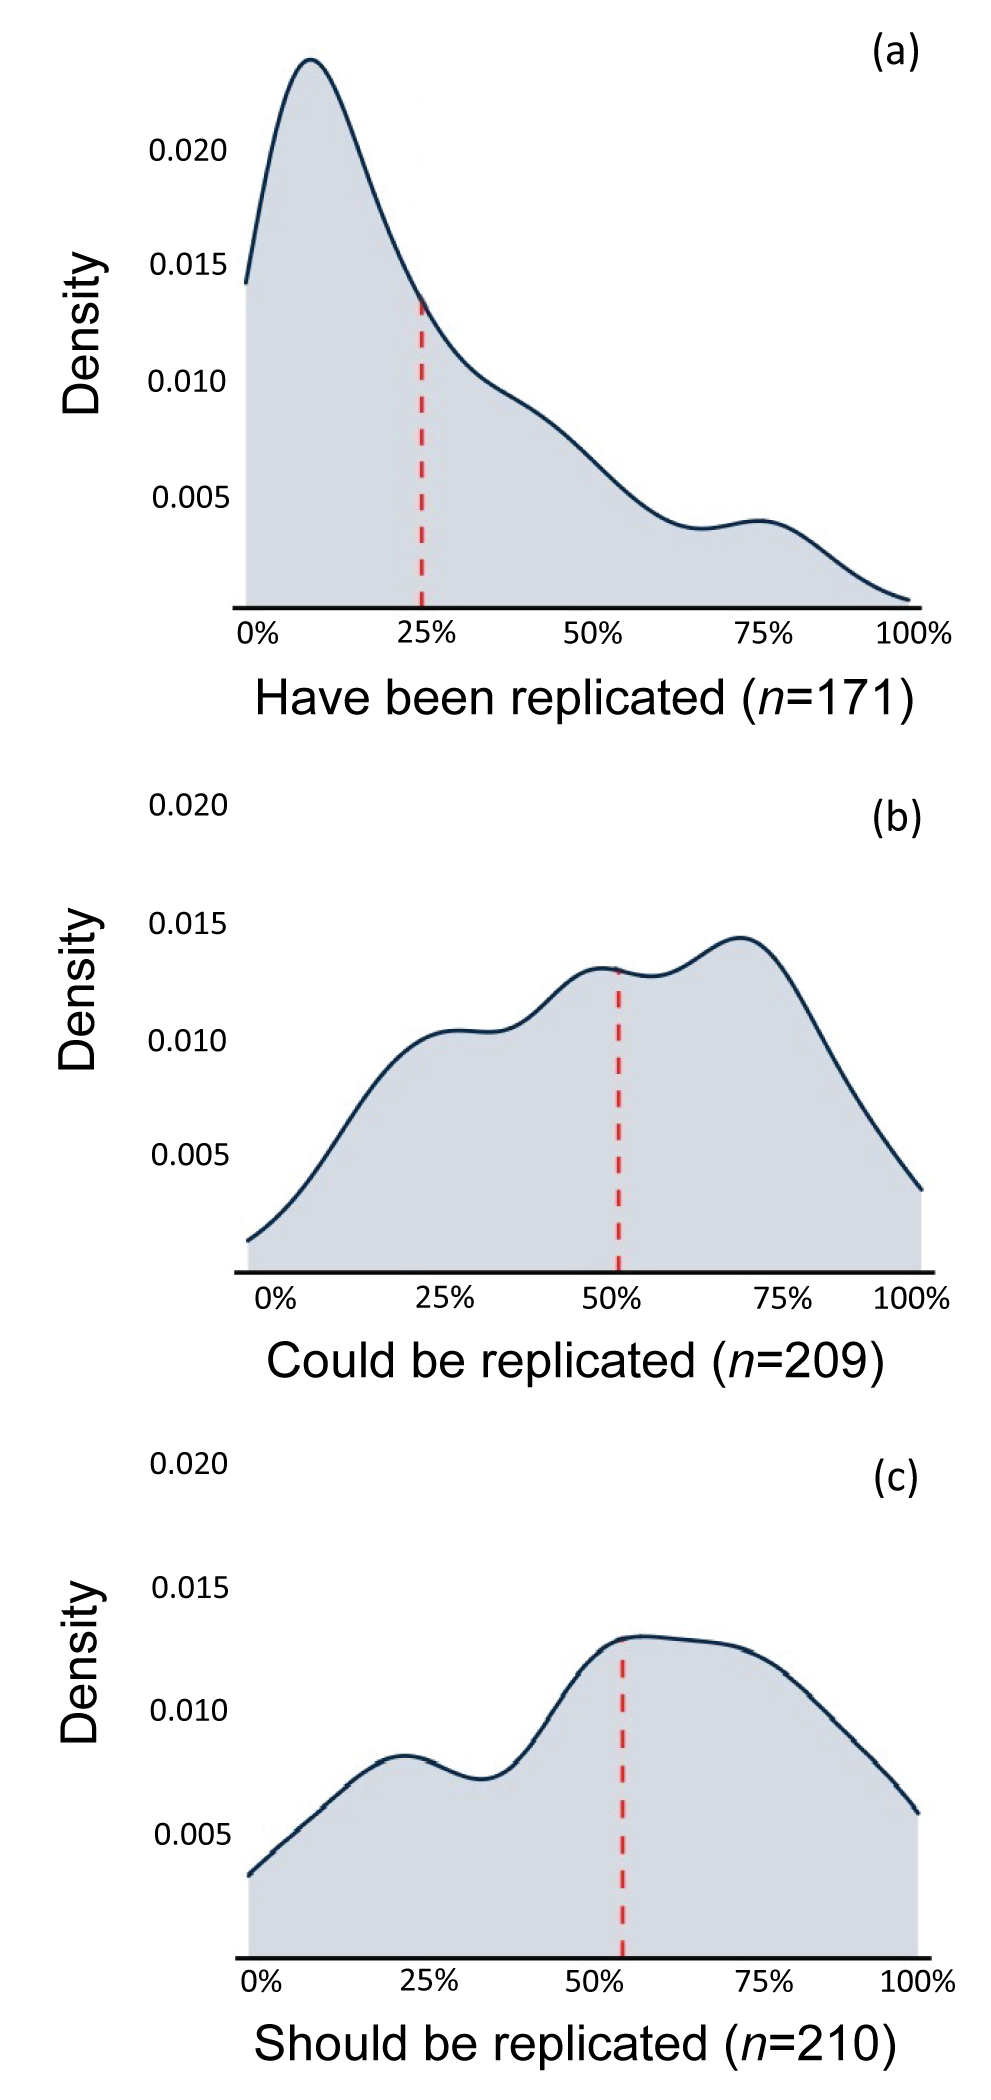
\includegraphics[scale=0.5]{results/figures/Fig-Q12-HCS.png}
    \caption{Estimates of the percentage of geographic studies that (a) have been replicated, (b) could be replicated, or (c) should be replicated}
    \label{fig:Q12-HCS}
\end{figure}

%%%%%%%%%%%%%%%%%%%%
\newpage

\begin{figure}[hbt!]
    \centering
    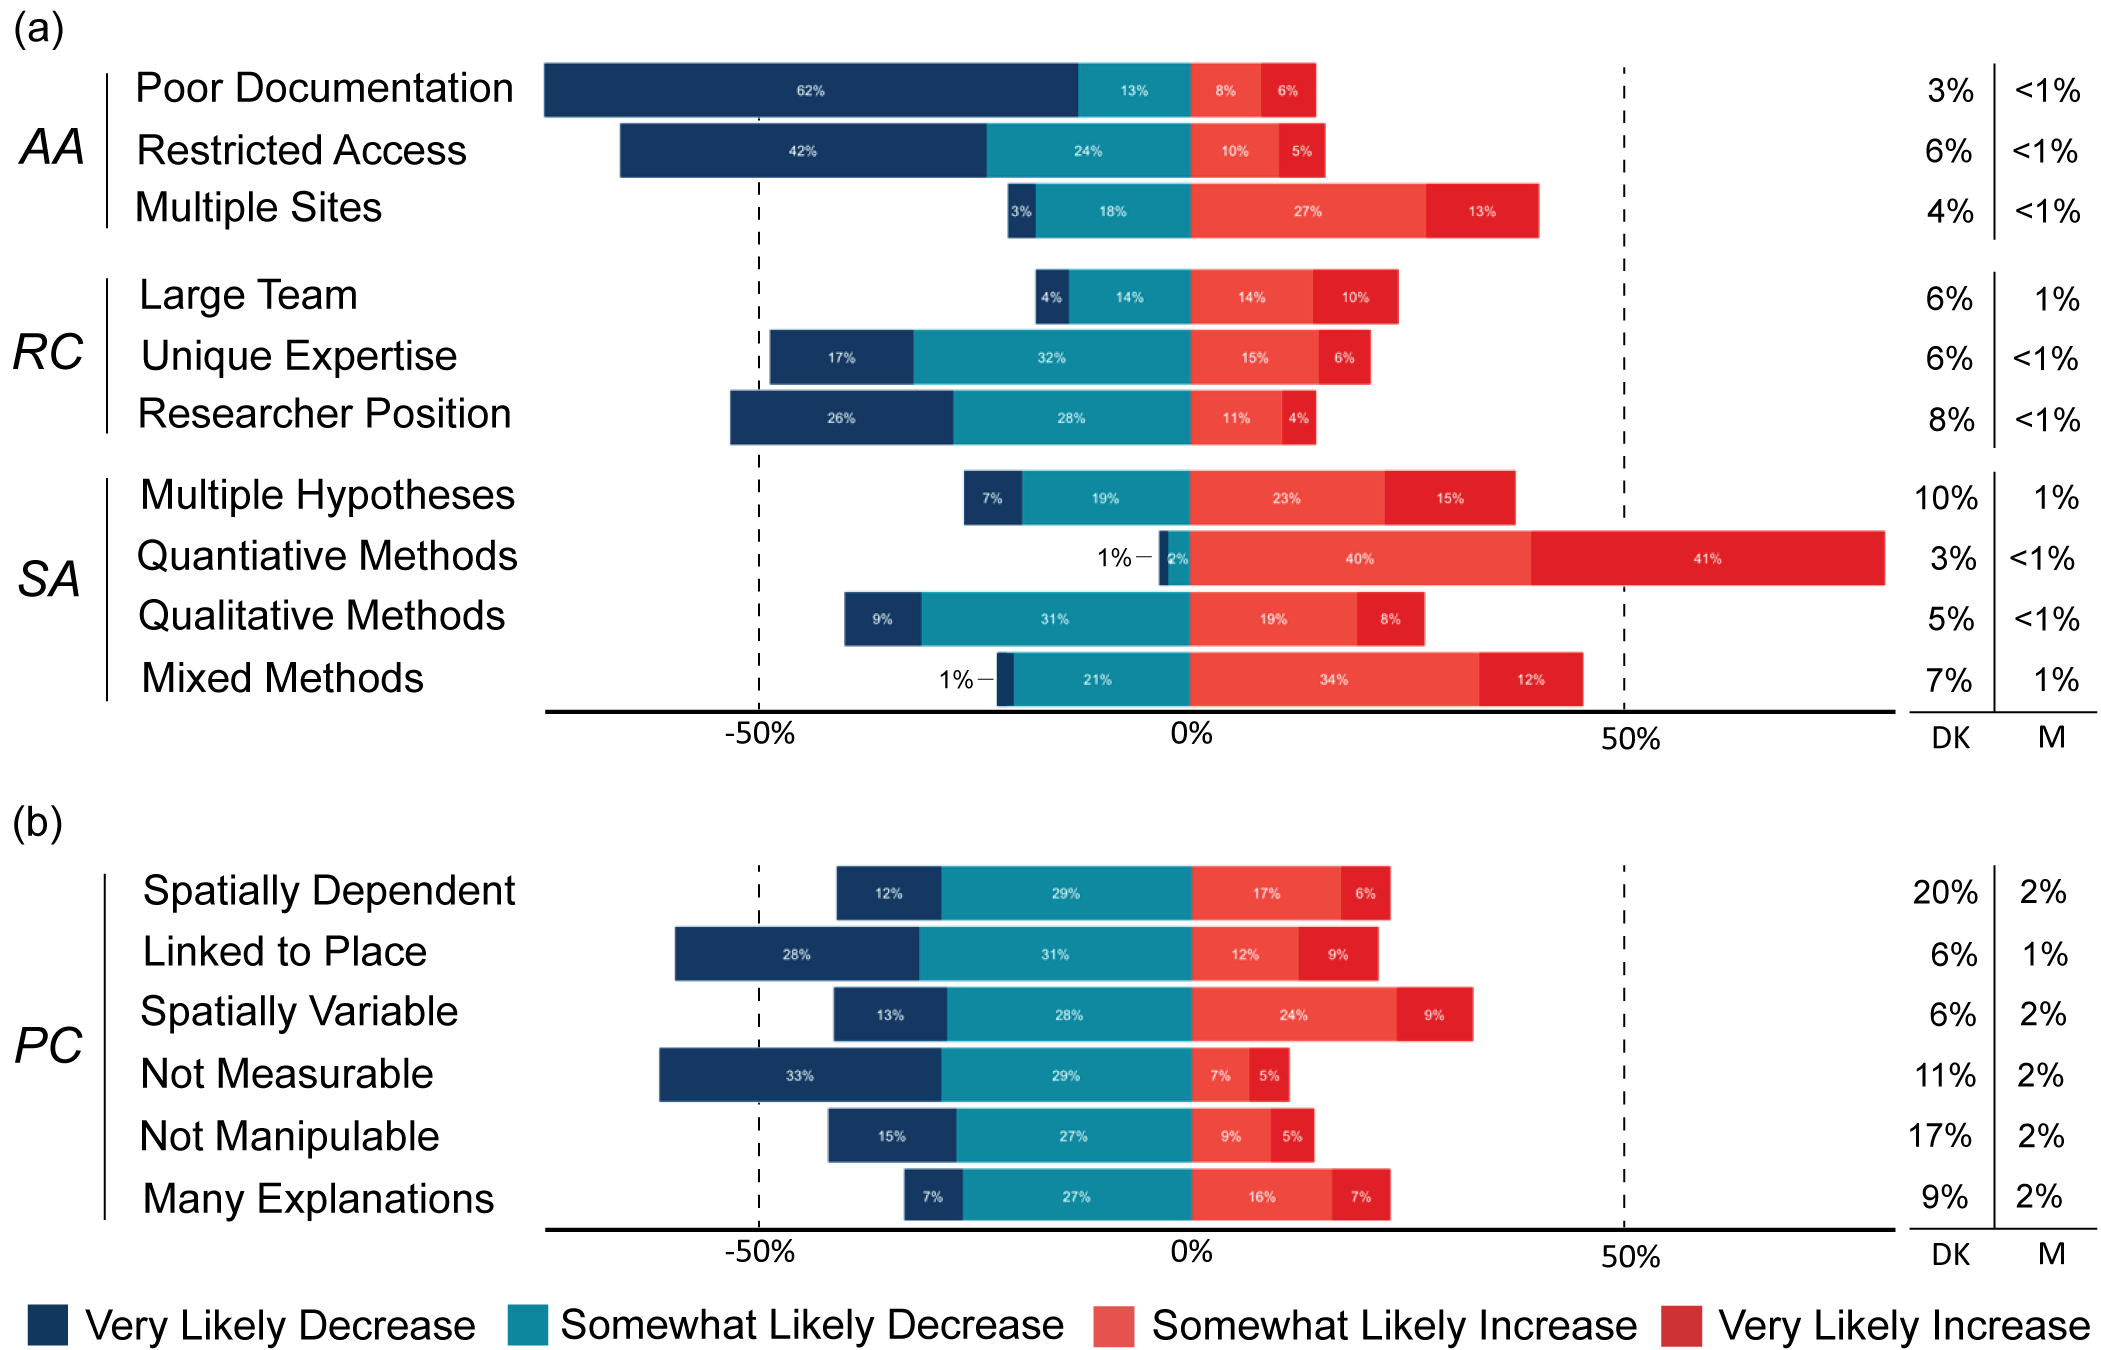
\includegraphics[scale=0.8]{results/figures/Fig-Q8-10-Chances.png}
    \caption{Factors affecting the chances of replicating a study. Respondents identified (a) how likely study characteristics were to alter the chances of successfully replicating a study and (b) how likely the characteristics of the phenomenon under investigation were to alter the chances of successfully replicating a study in a new location. Acronyms indicate: artifact accessibility (AA), researcher characteristics (RC), study approach (SA), and phenomenon characteristics (PC); and the percentage of `don't know' (DK) and missing (M) responses. Unlikely to affect replication chances is omitted, but can be calculated from available data.}
    \label{fig:Q8-10-Chances}
\end{figure}

%%%%%%%%%%%%%%%%%%%%
\newpage

\begin{figure}[hbt!]
    \centering
    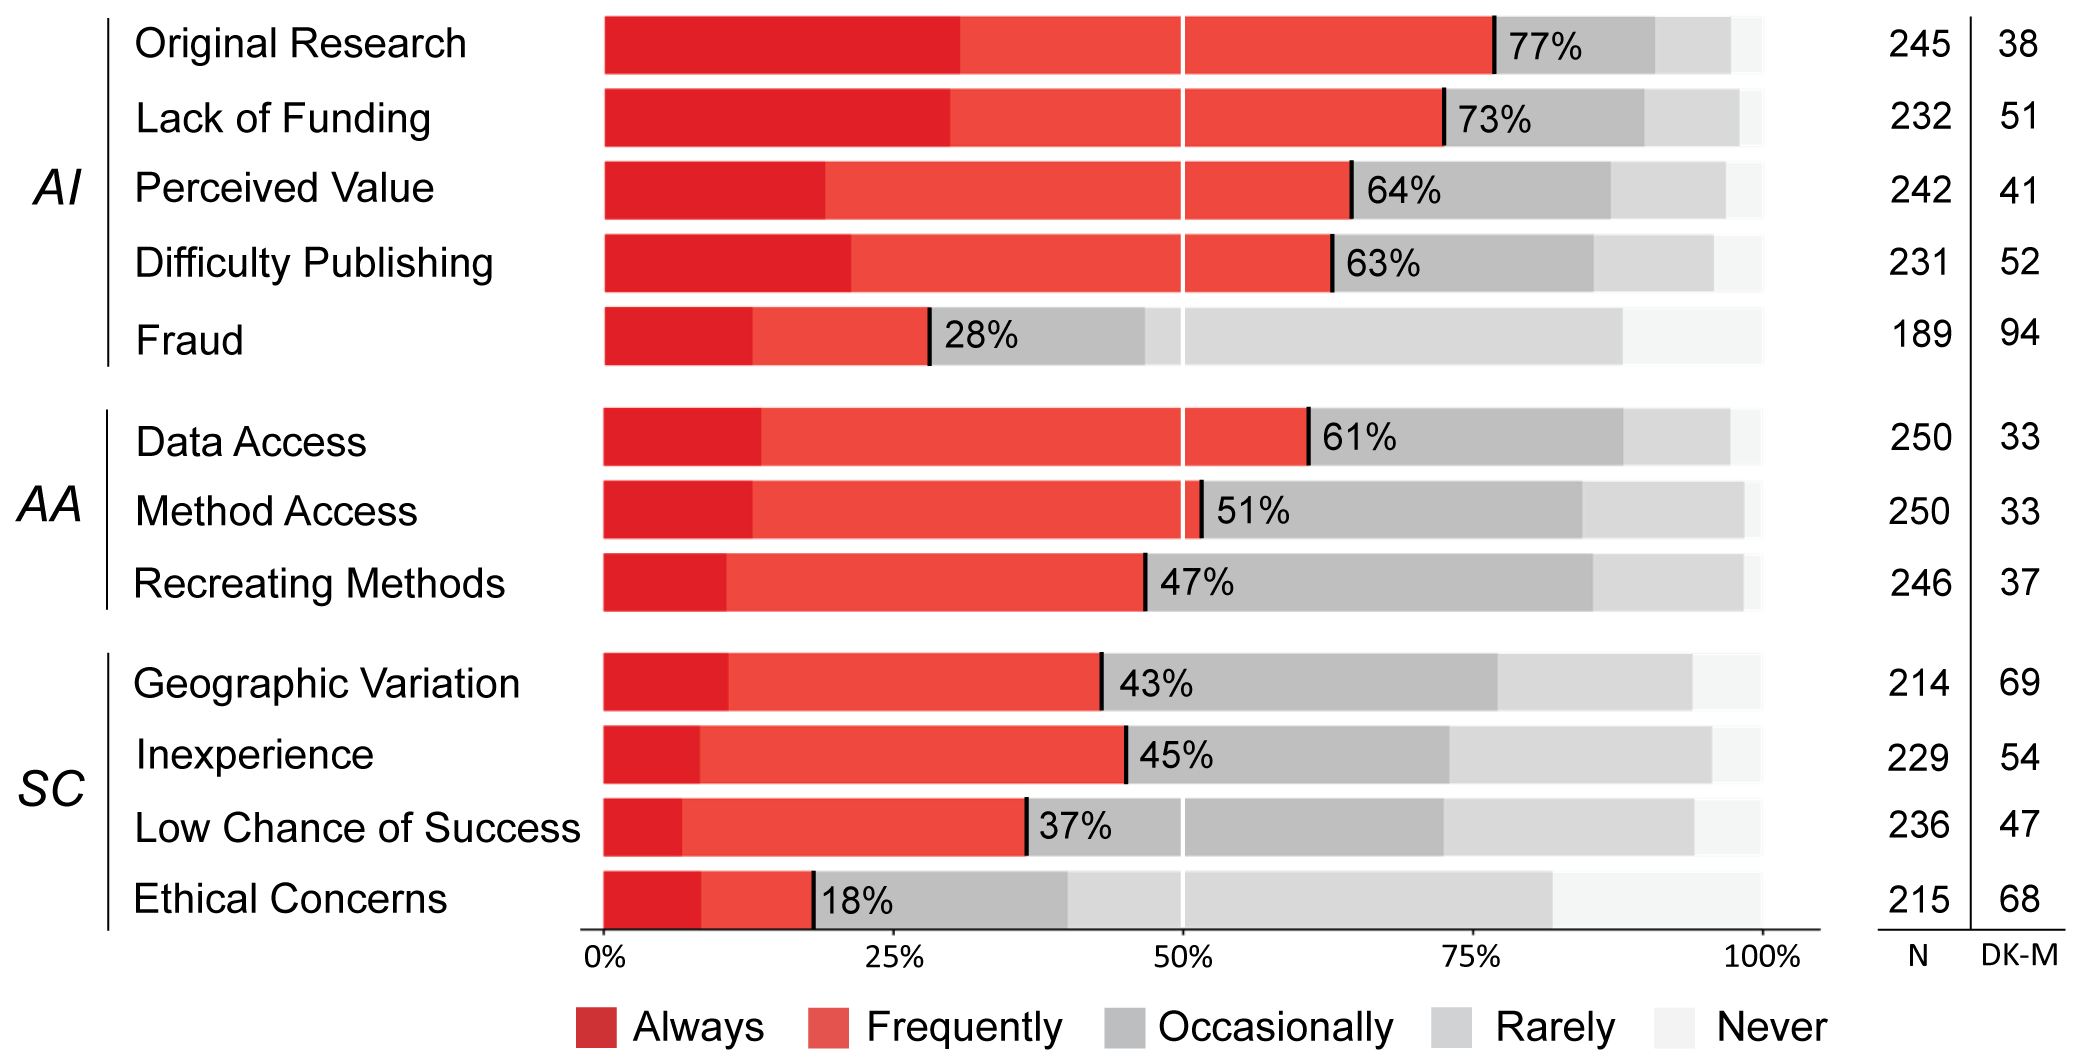
\includegraphics[scale=0.80]{results/figures/Fig-Q15-Decisions.png}
    \caption{Factors Affecting Researcher Decisions to Undertake Replication Studies. Factors grouped by: Academic Incentives (AA), Artifact Accessibility (AA), Study Characteristics (SC).}
    \label{fig:Q15-DecisionFactors}
\end{figure}

%%%%%%%%%%%%%%%%%%%%
\newpage
\noindent PETER KEDRON is an Associate Professor in the School of Geographical Science and Urban Planning and core faculty member in the Spatial Analysis Research Center (SPARC) at Arizona State University, Tempe, AZ, 85283, US. Email: Peter.Kedron@asu.edu. His research interests include spatial analysis, geographic information science, economic geography, and the accumulation of knowledge about geographic phenomena. \\  
  
\noindent JOSEPH HOLLER is an Assistant Professor of Geography at Middlebury College, Middlebury, VT, 05753, US. Email: \\
  
\noindent SARAH BARDIN is a PhD candidate ...

\end{document}